\documentclass[a4paper,12pt]{article}
\usepackage[utf8]{inputenc}
\usepackage{amsmath}
\usepackage{graphicx}
\usepackage{fancyhdr}
\usepackage{hyperref}
\usepackage{tocloft}

% Page formatting
\pagestyle{fancy}
\fancyhf{}
\fancyhead[L]{TEAM19}
\fancyhead[R]{October 8, 2023}
\fancyfoot[C]{\thepage}

\title{Bid for [P2024-04]}
\author{TEAM03}
\date{October 8, 2024}

\begin{document}

\maketitle

\tableofcontents
\newpage

\section{Introduction}
% Introduction content goes here
Our team is very interested to develop an innovative motion capture system based on multi-sensor fusion and artificial intelligence. Our group consists of skillful individuals with a strong foundation in programming, computer science, and other related skills, we are interested to explore the intersection of sensor technology and AI. With our group members expertise in Python, OpenCV, and PyTorch, along with a deep understanding of software engineering and image processing, we aim to integrate AI techniques with sensor data for enhanced accuracy and real-time performance.

This project will aligns very perfectly with our passion for combining artificial intelligence, robotics, and sensor technology to deliver an even more precise and efficient motion capture systems. We are very keen to undertake this challenge, leveraging deep learning algorithms and visualization techniques to develop a system that can have significant applications in various fields such as robotics, animation, and industrial automation. Our goal is to create a user-friendly, and high-performance motion capture system that pushes the boundaries of current technology.
\newpage
\section{Teammates}
    \subsection{Youyao Gao}
    \subsection*{Personal Information}
    \textbf{Student ID:} 20516639 \\
    \textbf{Email:} scyyg6@nottingham.edu.cn/youyaogao@gmail.com
    
    \subsection*{Introduction}
    I'm Youyao Gao, from Shanghai, a computer science student with a strong foundation in artificial intelligence in UNNC. With a robust educational background and a passion for technology, I have developed a keen interest in AI and machine learning, complemented by hands-on experience in both front-end and back-end development. Driven by curiosity and a continuous desire to learn, I'm eager to apply my technical skills and innovative thinking in a dynamic environment that challenges me to grow and contribute to advancements in technology.
    
    \subsection*{Internship Experience}
    \textbf	Algorithm Engineer of Shanghai Big Data Co., Ltd.
    
    \subsection*{Project Experience}
    \textbf Predicting Men's 100m Rankings at the Paris Olympics \\
    May -- July 2024
    
    \subsection*{Skill Set}
    \begin{itemize}
        \item \textbf{Programming Languages:} Python, C, java, Haskell, SQL, HTML, CSS, R
        \item \textbf{Interested area:} Software Engineering, AI, Financial Quantification
    \end{itemize}
    
    \subsection{Tongchang Liu}
    \subsection*{Personal Information}
    \textbf{Student ID:} 20513017 \\
    \textbf{Email:} scytl5@nottingham.edu.cn
    
    \subsection*{Introduction}
    I am Tongchang Liu, from Tianjin, a junior computer science student . I am keen on designing UI interfaces and making prototype. At the same time, I have some experience in using of sql language and excel table to process data and using python. Additionally, I am interested in Working with my teammates to learn more software engineering knowledge.
    
    \subsection*{Internship Experience}
    \textbf	NSCC-TJ\\
    \textbf Carbon Road Technology Co. LTD\\
    
    
    \subsection*{Skill Set}
    \begin{itemize}
        \item \textbf{Programming Languages:} Python, C, java, Haskell, SQL, HTML
        \item \textbf{Office skills:} Excel, PPT, Word, Adobe Photoshop, Git, Figma
    \end{itemize}
    
    \subsection{Ziqi Li}
    \subsection*{Personal Information}
    \textbf{Student ID:} 20514283 \\
    \textbf{Email:} scyzl13@nottingham.edu.cn
    
    \subsection*{Introduction}
    I am a junior student in computer science. I have some experience in Machine Learning, Java programming in back-end and also handle a little skill on front development such as webpage making.
    
    \subsection*{Internship Experience}
    \textbf{Software Engineer in CMB Network Technology Company} \\
    Jun -- Aug 2024
    
    \subsection*{Project Experience}
    \textbf{Modern Data Visualization of Big Data Research Seminar} \\
    May -- July 2024
    
    \subsection*{Skill Set}
    \begin{itemize}
        \item \textbf{Programming Languages:} Java, Python, Haskell, C, HTML, CSS, JavaScript, SQLite
        \item \textbf{Software:} IntelliJ IEDA, PyCharm, Anaconda, Visual Paradigm, Axure PR, LaTeX, MATLAB
    \end{itemize}
    
    \subsection{Yuhang Wu}
    \subsection*{Personal Information}
    \textbf{Student ID:} 20513290 \\
    \textbf{Email:} scyyw20@nottingham.edu.cn
    
    \subsection*{Introduction}
    I’m a third-year computer science student interests in coding and software development. Moreover, I am quite interested in artificial intelligence and robotics. I am willing to participate in team discussions with enthusiasm. I hope to develop my adaptability and time management skills in the project, learn relevant knowledge and improve my professional level.
    
    \subsection*{Internship Experience}
    \textbf{Hydrological modelling for flood estimation}  \\May 2024-Oct 2024
    \subsection*{Skill Set}
    \begin{itemize}
        \item \textbf{Programming Languages:} Java, Python, C, Haskell and MIPS Assembly.
        \item \textbf{Data Analysis based on:} Matlab, mySQL, Virtuoso Triplestore.
        \item \textbf{Front-end Platform:} Protégé.
        \item \textbf{Other Tools:} LaTeX.
    \end{itemize}
    \subsection{Shuqi Lee}
    \subsection*{Personal Information}
    \textbf{Student ID:} 20611680 \\
    \textbf{Email:} hcysl7@nottingham.edu.cn
    
    \subsection*{Introduction}
    I'm an exchange student from Nottingham Malaysia Campus,  with a strong passion for technology and a keen willingness to continuous learn new knowledge. Possessing a solid understanding of both frontend and backend development. Interested in AI and Machine Learning.
    
    \subsection*{Project Experience}
    \begin{itemize}
    \item \textbf {FOOD ORDERING WEBSITE}
    \item \textbf {2D PIXEL GAME}
    \item \textbf {Google Workspace Hackathon}
    \end{itemize}
    \subsection*{Skill Set}
    \begin{itemize}
        \item \textbf{Programming Languages:} Javascript, Java, C, Haskell, PHP, SQL.
        \item \textbf{Interested area:} AI, Machine Learning, Mobile Application
    \end{itemize}
    \subsection{Jason WIDJAYA}
    \subsection*{Personal Information}
    \textbf{Student ID:} 20512013 \\
    \textbf{Email:} scyjw13@nottingham.edu.cn
    
    \subsection*{Introduction}
    I am a junior student in Computer Science and Artificial Intelligence (CSAI) at the University of Nottingham
    Ningbo China. I have a strong interest in Virtual Reality (VR), Augmented Reality (AR), and Mixed Reality
    (MR). Additionally, I possess skills in graphical editing.
    
    
    \subsection*{Project Experience}
    \textbf Sept 2023 – Now
    V-ROOM Internship, University of Nottingham, Ningbo, China\\
    \textbf Developing Augmented Reality applications using Microsoft HoloLens\\
    \subsection*{Skill Set}
    \begin{itemize}
        \item \textbf{Programming Languages:} Python, Java, C, C\#, Unity, Haskell, MIPS Assembly languages.
        \item \textbf{Data Analysis:} MATLAB, SQLite, MySQL, Git, Flask
        \item \textbf{Other Tools:} LATEX, HTML, CSS
    \end{itemize}
\newpage

\section{Ideas \& Design}
\subsection{Our initial proposal for the game}
We aims to develop an innovative motion capture system that will leverages array of sensors sensors that is strategically positioned and artificial intelligence capability. This solution can be scalable, allowing applications in various industries, such as animation, robotics and automation. The goal is to provide an accesible motion tracking system using standard industrial cameras and sensors, enhanced by Artificial Intelligence and Deep Learning techniques.

The project will incorporate cutting-edge technology to fuse sensor data (cameras, IMUs) and apply advanced AI models for motion tracking, prediction, and visualization.



% Content for the initial proposal goes here
\subsection{Possible Tech Stack \& Primitive System design}
\begin{enumerate}
    \item Back-end Development

 Backend will use Python for the primary language as long as C++ for critical task. Key libraries will include OpenCV for image processing, PyTorch for AI model training
    \item Front-end Development
For the front-end development, we cam use unity or unreal engine for the 3D visualization. while we can use Flask or Django to provide the web UI for the user controls and experience. We can also use OpenGL for 3D visualization. Deep learning models such as CNNs and RNNs will handle the image recognition and motion prediction from the pre-trained models.
\end{enumerate}

\newpage

\section{Timeline \& Workflow and Work Distribution}
\subsection{Timeline \& Workflow}
% Content for Timeline \& Workflow goes here
\begin{itemize}
  \item \textbf{October 16 - October 31}
    \begin{itemize}
        \item \textbf{week 1-2:} Gather relevant literature, define equipment requests and complete ethics forms.
    \end{itemize}

    \item \textbf{November 1 - November 7}
    \begin{itemize}
        \item \textbf{week 3:} Define project requirements and identify the applications that will be used.
    \end{itemize}

    \item \textbf{November 8 - November 21}
    \begin{itemize}
        \item \textbf{week 4-5:}  Design the system architecture and begin coding implementations.
    \end{itemize}
    
    \item \textbf{November 22 - December 5}
    \begin{itemize}
        \item \textbf{week 6-7:}  Test the model, perform simple preliminary image processing and also, complete an interim report.
    \end{itemize}
    \item \textbf{December 5 - January 16}
    \begin{itemize}
        \item \textbf{week 8-14:}  Develop a detailed system architecture, develop the data collection and preprocess module, implement model selection and architecture setup.
    \end{itemize}
    \item \textbf{January 17 - February 20}
    \begin{itemize}
        \item \textbf{week 15-20:}  Train the deep learning model, validate model accuracy and the responsiveness of real-time applications.
    \end{itemize}
    \item \textbf{February 21 - March 20}
    \begin{itemize}
        \item \textbf{week 21-25:}  Integrate the system, develop the user interface, and perform comprehensive system testing.
    \end{itemize}
    \item \textbf{March 21 - April 2}
    \begin{itemize}
        \item \textbf{week 26-28:}  Complete project documentation and deploy the system.
    \end{itemize}

\end{itemize}

\subsection{Work Distribution}
% Content for Work Distribution goes here
To ensure the success of this project, we have divided the responsibilities among our team members as follows:
\begin{itemize}
    \item \textbf{Youyao Gao}:
    Responsible for designing and implementing the data collection module, especially sensor data.
    \item \textbf{Tongchang Liu,Ziqi Li}:
    In charge of selecting suitable deep learning models and conducting training.
    \item \textbf{Yuhang Wu,Shu Lee}:
    Handles the final integration and comprehensive testing of the system.
    \item \textbf{Jason Lymand WIDJAYA}:
    Develops intuitive user interfaces and data visualizations.
\end{itemize}
\begin{figure}[ht]
  \centering
  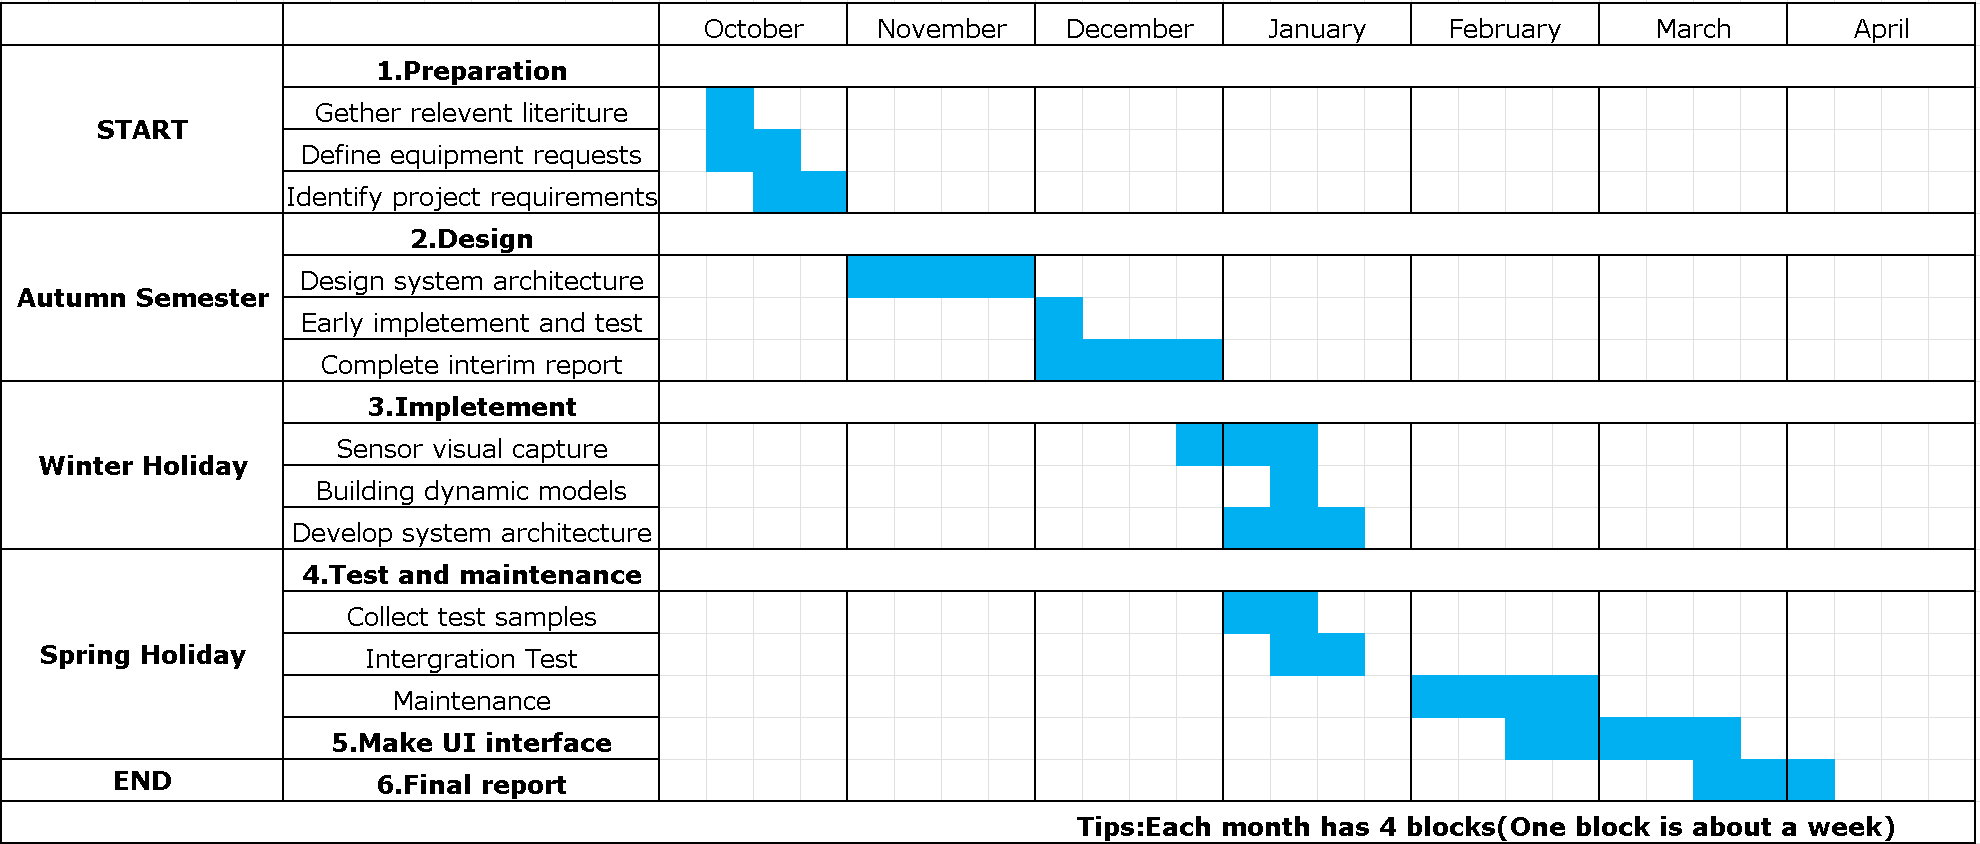
\includegraphics[width=\textwidth]{GRP-Timetable.png}
  \caption{Timetable}
  \label{fig:your_label}
\end{figure}
\newpage
\section{Conclusion}
% Conclusion content goes here
In this project, our team proposes to develop an innovative motion capture system based on multi-sensor fusion and artificial intelligence. By integrating advanced technologies like Python, OpenCV, and PyTorch, we aim to enhance the system's accuracy and real-time performance with AI techniques. This project aligns perfectly with our passion for merging AI, robotics, and sensor technology, pushing the boundaries of current technology to provide a precise and efficient motion tracking solution across various sectors, including robotics, animation, and industrial automation.

With the application of deep learning algorithms and visualization techniques, we plan to develop a user-friendly, high-performance motion capture system that can achieve significant practical impacts. The professional expertise and innovative drive of our team ensure the successful execution of this project.At the same time, this project can cultivate our ability to communicate and cooperate with each other, help us accumulate enough software engineering experience and expand our professional knowledge.
\end{document}
